\section{名前空間による整理}

Clojureコードは、一連の個々のトップレベル・フォーム(関数、レコード、プロトコルなど)としてコンパイルされ評価されますが、Clojureはそれらの個々のフォームをグループ化するための名前空間を提供します。名前空間は、フォームのグループを収集し、整理し、名前を付けるために使用できる、名前付きの階層的なコンテナです。名前空間の実用的な使い方の1つは、どこかで同じ名前と衝突することを心配することなく、コードで単純な名前を使えるようにすることです。名前空間は、どれを意味しているのかを指定する手段を提供します。

Clojureのコードはより細かい要素で構成されていますが、依存関係は関数レベルではなく、名前空間レベルで宣言され、読み込まれます。各名前空間の \texttt{ns} マクロは、その依存関係を定義し、まとめて依存関係グラフを作成する。この依存関係グラフは、名前空間がロードされる順序に影響を与える。名前空間がマルチメソッドやプロトコル(いずれも型固有の動作のためのオープンシステム)の実装を提供する場合、実装を使用する前にロードする必要があるため、このロード順序が重要になることがあります。

名前空間とコンポーネントは、どちらも組織化のためのツールである。名前空間は機能を整理するための言語機能であり、コンポーネントは問題レベルで整理するための手段である。この2つのアプローチは、どちらも有用であり、連動してコードを構造化し、最終的に他の開発者が理解しやすく、使いやすくするものです。

\subsection{名前空間のカテゴリ}

Clojureで関数のセットを名前空間にグループ化するのは、多くの理由があります。以下のカテゴリは、アプリケーションを反映した論理的な名前空間アーキテクチャを作成するために使用することができます。

\begin{description}
\item [Utility] utility名前空間は、ドメインや目的別に整理された汎用的な関数を提供します。例えば、文字列操作や特定のファイル形式の解析のための名前空間を作成することができます。一般に、utility名前空間は依存関係がほとんどありません。
\item [Data definition] カスタムコレクションやドメインエンティティのセットを、コレクションやエンティティを使用するためのヘルパー関数と一緒にネームスペースで定義するのが一般的である。
\item [Abstraction] プロトコルのような抽象的なものは、最小限の依存関係でネームスペースに分離することができます。
\item [Implementation] 一方、プロトコルやインタフェースで定義された抽象化機能を名前空間で実装すると便利なことが多い。この実装は、アプリケーションに組み入れることができる。
\item [Assembly] 実装のセットと、実装をどのように構築し接続するかを指定する構成がある場合、assembly名前空間がすべてを結びつけます。実装の内部では、一般に抽象化(プロトコル)またはデータ構造のみが直接使用される。
\item [Entry point] ほとんどのアプリケーションには、アプリケーションの開始(設定の収集を含む)とアセンブリや他のライフサイクル操作の開始をつなぐ1つ以上のエントリーポイントがあります。
\end{description}

次の図は、ライブラリやアプリケーションの中で、これらの種類の名前空間がどのように一般的に重なり合っているかを示しています。

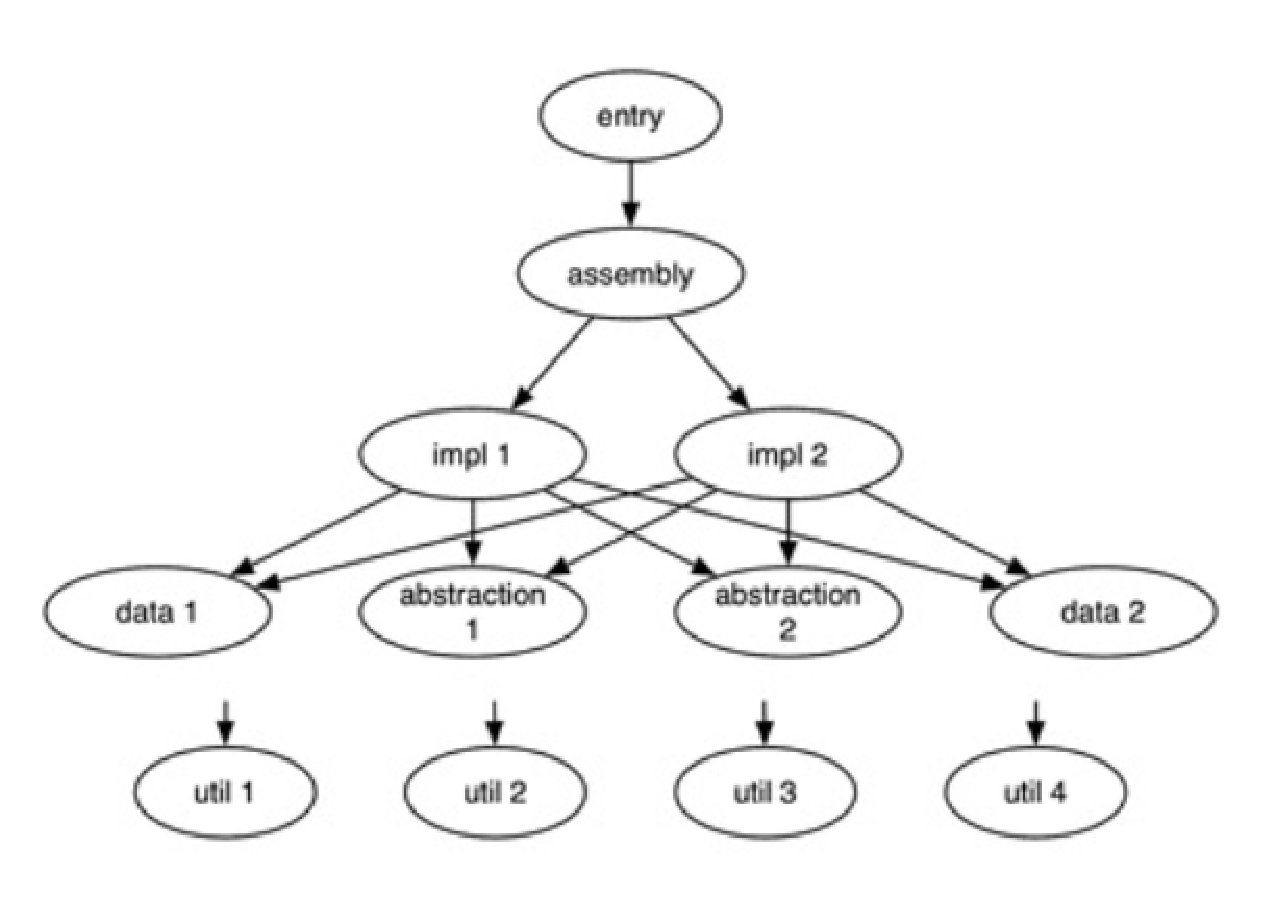
\includegraphics[width=10cm]{fig_06_001.eps}

この構造は、独自の名前空間構造を設計する際のガイドラインとして有効である。ユーティリティ名前空間は依存関係グラフの一番下にあり、それ自身の依存関係はほとんどなく、上の複数の名前空間によって使用されています。次の層は、データまたは抽象化名前空間のいずれかからなり、アプリケーション自体のビルディングブロックを作成します。抽象化の上には、その抽象化のための実装があります。その上には、設定が処理され、実装が組み立てられて接続され、 アプリケーションの状態が作成されるアセンブリ層があります。一番上には、ウェブアプリケーション、コマンドラインインターフェース、サービスなど、一つまたは複数のエントリーポイントがあります。

プロジェクト内の名前空間を名前空間ツリーとして整理するには、さまざまなアプローチがありますが、唯一の正解はありません。小規模なプロジェクトでは、ネームスペースの大部分をプロジェクトにちなんだ単一のルート内に配置し、ネストを最小限にすることがよくあります。

\begin{lstlisting}[numbers=none]
myproject.util.string ;; utility
myproject.util.json ;; utility
myproject.domain    ;; data - domain entities
myproject.config    ;; data - config data
myproject.services  ;; abstraction - service definitions
myproject.impl.xyz  ;; implementation of service abstraction
myproject.assembly  ;; assembly
myproject.main      ;; main entry point - command-line
\end{lstlisting}

小規模なシステムでは、多くの抽象化機能、実装、ユーティリティをグループ化して、サービスを水平方向に切り分けるのが最も簡単な場合があります。システムが大きくなるにつれて、システムを縦割りにして、それぞれのコンポーネントをAPI、実装、データ定義のセット、ユーティリティで構成することがますます有用になってきます。

\subsection{パブリックとプライベートの関数}

Clojureは、データや関数をデフォルトで利用できるようにすることに偏っています。しかし、ほとんどの名前空間には、ヘルパーとして使用される関数や、決して一般的な使用方法の一部となることを意図していない関数があります。名前空間内の関数を定義するときは、消費者がそれらの関数をどのように認識し、どのように使用することが期待されるかを考えてください。いくつかのツールや規約は、プライベートvar、ドキュメント文字列、そして名前空間の構造そのものです。

Clojureに組み込まれた主要なツールは、 \texttt{defn-} または \texttt{\^:private} メタタグを使用して関数をプライベートとしてマークする機能です。


\begin{lstlisting}[numbers=none]
(defn- internal-function [] ...)
(def ^:private internal-constant 42)
\end{lstlisting}


これらのvarはいくつかの名前空間関数の結果から省略されますが、それでもreader var構文で直接アクセスしたり、名前空間オブジェクトを直接呼び出したりすることは可能です。

autodocのようなドキュメント生成ツールは、docstringを持たない関数を省略することがあります。Clojureコア自身は、高度なClojure開発には有用ですが、一般的な使用には適さない内部関数を強調しないためにこの機能を使用します。

最後に、 \texttt{myproject.internal.db} のような名前空間を使用して、内部であることを明示的にマークするのはよくあることで、 \texttt{internal} 以下のすべての名前空間は非パブリックとみなされます。

これらのテクニックは、自分のコードの利用者にどこから手をつければよいかを示すのに役立つと思われます。

さて、名前空間をどのように整理すればいいのかがわかったところで、 それらの名前空間を使っていくつかのコンポーネントを作成してみましょう。まずはコンポーネントのAPIをどのように設計するかを考えてから、コンポーネントをどのように実装するかを考えていきます。






